\documentclass[12pt, varwidth, border={20mm 5mm 5mm 20mm}]{standalone}
\usepackage{tikz}
\usepackage{amsmath}
\usepackage[a4paper, portrait, margin=1cm]{geometry}
\begin{document}
\section*{Forces}
\begin{minipage}{0.4\textwidth}
    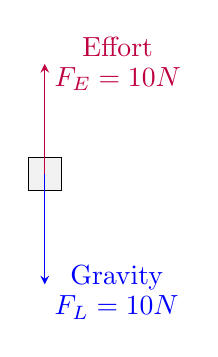
\begin{tikzpicture}[scale=0.7,>=stealth]
        % First class lever
        %load
        \draw[fill=gray!10] (-0.3,0.0) rectangle (0.3,0.6);
        \draw[->,blue,thin] (0.0,0.3) -- (0.0,-1.7) node[below,right,yshift=-0.1cm,align=center] {Gravity \\\\[-3ex] $F_L = 10N$};
        %effort
        \draw[->,purple,thin]  (0.0,0.3) -- (0.0,2.3) node[above,right,align=center] {Effort \\\\[-3ex] $F_E = 10N$};

    \end{tikzpicture}
\end{minipage}%
\hfill
\begin{minipage}{0.4\textwidth}
    \begin{align*}
        % forces
         net force &={F_E} - {F_L} \\\\
         &=10N - 10N \\\\
         &=0N
    \end{align*}
\end{minipage}
\end{document}
